\documentclass[aspectratio=169, 12pt]{beamer}

% Minimal clean theme
\usetheme{default}
\usecolortheme{default}

% Remove navigation symbols and other clutter
\setbeamertemplate{navigation symbols}{}
\setbeamertemplate{footline}[frame number]
\setbeamertemplate{frametitle}{\vspace{1em}\insertframetitle}

% Clean fonts
\usefonttheme{serif}

% Lots of white space
\setbeamersize{text margin left=1.5cm, text margin right=1.5cm}

% Packages
\usepackage[utf8]{inputenc}
\usepackage{graphicx}
\usepackage{amsmath}
\usepackage{amssymb}
\usepackage{hyperref}
\usepackage{multirow}
\usepackage{booktabs}
\usepackage{xcolor}
\usepackage{listings}
\usepackage{tikz}

% Settings
\graphicspath{{./assets/}{../assets/}{../../assets/}}

% Title page info
\title{Federated Learning for Industrial Anomaly Detection}
\subtitle{Stage 1: Baseline Development \& Independent Client Setup}
\author{AI for Trustworthy Decision Making}
\institute{AutoVI Dataset Project}
\date{\today}

% Custom colors
\definecolor{darkblue}{rgb}{0, 0.2, 0.6}
\definecolor{darkgreen}{rgb}{0, 0.4, 0}
\definecolor{darkred}{rgb}{0.6, 0, 0}

% ============================================================================
\begin{document}

% ============================================================================
% Slide 1: Title Slide
% ============================================================================
\frame{\titlepage}

% ============================================================================
% Slide 2: Problem & Motivation
% ============================================================================
\begin{frame}
\frametitle{The Challenge: Privacy in Industrial Quality Control}

\begin{columns}[T]
    \column{0.5\textwidth}
    \textbf{Current Problem:}
    \begin{itemize}
        \item Manufacturing data is \textcolor{darkred}{proprietary}
        \item Different factories = \textcolor{darkred}{isolated data}
        \item Regulatory \textcolor{darkred}{restrictions} on data sharing
        \item Cannot train shared models easily
    \end{itemize}

    \column{0.5\textwidth}
    \vspace{2em}
    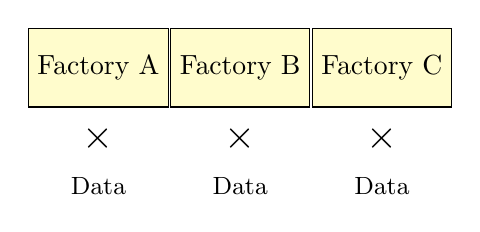
\begin{tikzpicture}[scale=0.6]
        % Factories
        \node[draw, rectangle, minimum width=1.5cm, minimum height=1cm, fill=yellow!20] at (0,2) {Factory A};
        \node[draw, rectangle, minimum width=1.5cm, minimum height=1cm, fill=yellow!20] at (3,2) {Factory B};
        \node[draw, rectangle, minimum width=1.5cm, minimum height=1cm, fill=yellow!20] at (6,2) {Factory C};

        % Data icons
        \node at (0,0.5) {\Large $\times$};
        \node at (3,0.5) {\Large $\times$};
        \node at (6,0.5) {\Large $\times$};

        % Labels
        \node[text width=1.5cm, align=center, font=\small] at (0,-0.5) {Data};
        \node[text width=1.5cm, align=center, font=\small] at (3,-0.5) {Data};
        \node[text width=1.5cm, align=center, font=\small] at (6,-0.5) {Data};
    \end{tikzpicture}
\end{columns}

\vspace{1.5em}
\hrule

\vspace{1em}
\textbf{\Large Solution: Federated Learning}

{\large \textcolor{darkgreen}{\checkmark}} Train models \textbf{locally}, share only \textbf{model updates}\\
{\large \textcolor{darkgreen}{\checkmark}} No raw data leaves the facility\\
{\large \textcolor{darkgreen}{\checkmark}} Preserve privacy while enabling collaboration

\end{frame}

% ============================================================================
% Slide 3: Dataset Overview - AutoVI
% ============================================================================
\begin{frame}
\frametitle{Dataset: Automotive Visual Inspection (AutoVI)}

\textbf{Real industrial data from Renault Group}

\vspace{1em}
\begin{columns}[T]
    \column{0.5\textwidth}

    \textbf{6 Product Categories:}
    \begin{itemize}
        \item engine\_wiring (285 train)
        \item pipe\_clip (195 train)
        \item pipe\_staple (191 train)
        \item tank\_screw (318 train)
        \item underbody\_pipes (161 train)
        \item underbody\_screw (373 train)
    \end{itemize}

    \column{0.5\textwidth}

    \textbf{Dataset Statistics:}
    \begin{table}[H]
    \small
    \begin{tabular}{rc}
    \toprule
    \textbf{Metric} & \textbf{Value} \\
    \midrule
    Total Images & 3,950 \\
    Training Images & 1,523 \\
    Test Images & 2,399 \\
    Categories & 6 \\
    Defect Types & 10 \\
    \bottomrule
    \end{tabular}
    \end{table}
\end{columns}

\vspace{1.5em}
\begin{tikzpicture}[overlay, remember picture]
    \node[anchor=south east, xshift=-1cm, yshift=1cm] at (current page.south east) {
        \textcolor{gray}{\small \% TODO: Insert image grid (6 categories)}
    };
\end{tikzpicture}

\begin{itemize}
    \item \textbf{Unsupervised setup}: Train on ``good'' images only
    \item \textbf{Real world}: Lighting variation, authentic defects
    \item \textbf{Pixel annotations}: Ground truth masks for localization
\end{itemize}

\end{frame}

% ============================================================================
% Slide 4: Baseline Model - PatchCore
% ============================================================================
\begin{frame}
\frametitle{Baseline Model: PatchCore Architecture}

\textbf{Memory Bank-Based Anomaly Detection}

\begin{columns}[T]
    \column{0.6\textwidth}

    \begin{enumerate}
        \item \textbf{Feature Extraction}
        \begin{itemize}
            \item Pre-trained WideResNet-50-2 backbone
            \item Multi-scale features (Layer 2 + Layer 3)
            \item Output: 1536-dim patch embeddings
        \end{itemize}

        \item \textbf{Memory Bank (Coreset)}
        \begin{itemize}
            \item Greedy selection (10\% of patches)
            \item Represents ``normal'' feature space
            \item Computationally efficient
        \end{itemize}

        \item \textbf{Anomaly Scoring}
        \begin{itemize}
            \item Distance to nearest bank feature
            \item Upsampled to pixel resolution
            \item Produces anomaly heatmaps
        \end{itemize}
    \end{enumerate}

    \column{0.4\textwidth}

    \textcolor{gray}{\% TODO: Architecture diagram}

    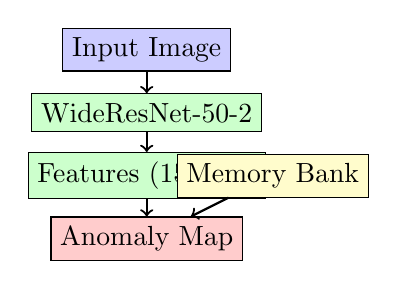
\begin{tikzpicture}[scale=0.8]
        % Input
        \node[draw, rectangle, fill=blue!20] (input) at (0,3) {Input Image};

        % Backbone
        \node[draw, rectangle, fill=green!20] (backbone) at (0,2) {WideResNet-50-2};
        \draw[->, thick] (input) -- (backbone);

        % Features
        \node[draw, rectangle, fill=green!20] (features) at (0,1) {Features (1536-D)};
        \draw[->, thick] (backbone) -- (features);

        % Memory bank
        \node[draw, rectangle, fill=yellow!20] (memory) at (2,1) {Memory Bank};

        % Scoring
        \node[draw, rectangle, fill=red!20] (score) at (0,0) {Anomaly Map};
        \draw[->, thick] (features) -- (score);
        \draw[->, thick] (memory) -- (score);
    \end{tikzpicture}
\end{columns}

\vspace{1em}
\hrule

\textbf{Why PatchCore?}
\begin{itemize}
    \item {\large \textcolor{darkgreen}{\checkmark}} State-of-the-art on MVTec AD and similar datasets
    \item {\large \textcolor{darkgreen}{\checkmark}} Memory bank can be aggregated (federated-friendly)
    \item {\large \textcolor{darkgreen}{\checkmark}} Interpretable anomaly maps for quality control
\end{itemize}

\end{frame}

% ============================================================================
% Slide 5: Federated Learning Setup - Stage 1
% ============================================================================
\begin{frame}
\frametitle{Federated Architecture: 5 Clients with IID Partitioning}

\textbf{Balanced data distribution across clients}

\begin{table}[H]
\centering
\small
\begin{tabular}{lccc}
\toprule
\textbf{Client} & \textbf{Samples} & \textbf{Patches} & \textbf{Coreset (10\%)} \\
\midrule
Client 0 & 305 & 59,780 & 5,978 \\
Client 1 & 305 & 59,780 & 5,978 \\
Client 2 & 305 & 59,780 & 5,978 \\
Client 3 & 304 & 59,584 & 5,958 \\
Client 4 & 304 & 59,584 & 5,958 \\
\midrule
\textbf{Total} & \textbf{1,523} & \textbf{298,508} & \textbf{29,850} \\
\bottomrule
\end{tabular}
\end{table}

\vspace{0.5em}
\textbf{IID Partitioning:} Each client receives samples from all 6 categories

\begin{itemize}
    \item \textbf{Balanced distribution}: $\sim$305 samples per client
    \item Each client has \textbf{mixed categories} (engine\_wiring, pipe\_clip, etc.)
    \item Local coreset selection: \textbf{10\%} of extracted patches
    \item Foundation for federated aggregation
\end{itemize}

\vspace{0.5em}
\textbf{Goal:} Simulate distributed factories with similar inspection tasks

\end{frame}

% ============================================================================
% Slide 6: Federated Memory Bank Aggregation
% ============================================================================
\begin{frame}
\frametitle{Federated Memory Bank Aggregation}

\begin{center}
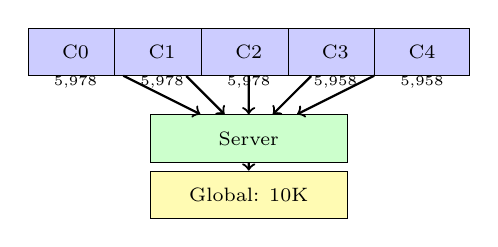
\begin{tikzpicture}[scale=0.55, every node/.style={font=\scriptsize}]
    % Stage 1: Local clients in a row
    \node[draw, rectangle, fill=blue!20, minimum width=1.2cm, minimum height=0.6cm] (c0) at (0,2.5) {C0};
    \node[draw, rectangle, fill=blue!20, minimum width=1.2cm, minimum height=0.6cm] (c1) at (2,2.5) {C1};
    \node[draw, rectangle, fill=blue!20, minimum width=1.2cm, minimum height=0.6cm] (c2) at (4,2.5) {C2};
    \node[draw, rectangle, fill=blue!20, minimum width=1.2cm, minimum height=0.6cm] (c3) at (6,2.5) {C3};
    \node[draw, rectangle, fill=blue!20, minimum width=1.2cm, minimum height=0.6cm] (c4) at (8,2.5) {C4};

    % Local coreset counts
    \node[font=\tiny] at (0,1.8) {5,978};
    \node[font=\tiny] at (2,1.8) {5,978};
    \node[font=\tiny] at (4,1.8) {5,978};
    \node[font=\tiny] at (6,1.8) {5,958};
    \node[font=\tiny] at (8,1.8) {5,958};

    % Server
    \node[draw, rectangle, fill=green!20, minimum width=2.5cm, minimum height=0.6cm] (server) at (4,0.5) {Server};

    % Arrows
    \draw[->, thick] (c0) -- (server);
    \draw[->, thick] (c1) -- (server);
    \draw[->, thick] (c2) -- (server);
    \draw[->, thick] (c3) -- (server);
    \draw[->, thick] (c4) -- (server);

    % Global bank
    \node[draw, rectangle, fill=yellow!30, minimum width=2.5cm, minimum height=0.6cm] (global) at (4,-0.8) {Global: 10K};
    \draw[->, thick] (server) -- (global);
\end{tikzpicture}
\end{center}

\begin{columns}[T]
    \column{0.5\textwidth}
    \textbf{Local Processing:}
    \begin{itemize}
        \item Extract 784 patches/image
        \item Coreset: 10\% selection
        \item Total: 29,850 patches
    \end{itemize}

    \column{0.5\textwidth}
    \textbf{Server Aggregation:}
    \begin{itemize}
        \item Weighted 2x oversampling
        \item Diversity selection
        \item Final: 10,000 patches
    \end{itemize}
\end{columns}

\vspace{0.5em}
\centering
\textbf{Compression:} 298K $\rightarrow$ 30K $\rightarrow$ 10K (\textbf{96.6\% reduction})

\end{frame}

% ============================================================================
% Slide 7: Aggregation Strategies
% ============================================================================
\begin{frame}
\frametitle{Aggregation Strategies}

\begin{table}[H]
\centering
\tiny
\begin{tabular}{lp{3cm}p{2.5cm}c}
\toprule
\textbf{Strategy} & \textbf{Description} & \textbf{Trade-off} & \textbf{Used} \\
\midrule
\textbf{Federated Coreset} & Weighted + oversampling + diversity & Fairness + diversity & \textcolor{darkgreen}{\checkmark} \\
Simple Concatenate & Direct merge & Fast, no fairness & \\
Diversity Preserving & Min. 100 patches/client & Small client voice & \\
\bottomrule
\end{tabular}
\end{table}

\textbf{Federated Coreset Algorithm:}
\begin{enumerate}
    \item Weight contributions by sample count
    \item Oversample 2x from each client
    \item Apply greedy coreset selection
\end{enumerate}

\textbf{Client Weights (IID):} $\sim$0.20 each

\vspace{0.5em}
\begin{center}
\fbox{\textit{Only embeddings shared -- raw images never leave clients}}
\end{center}

\end{frame}

% ============================================================================
% Slide 8: Experimental Setup & Training Stats
% ============================================================================
\begin{frame}
\frametitle{Experimental Setup \& Training Statistics}

\begin{columns}[T]
    \column{0.5\textwidth}
    \textbf{Configuration:}
    \begin{itemize}
        \item Clients: 5 (IID)
        \item Backbone: WideResNet50-2
        \item Features: layer2 + layer3
        \item Dimension: 1536
        \item Image: 224$\times$224
    \end{itemize}

    \column{0.5\textwidth}
    \textbf{Results:}
    \begin{itemize}
        \item Time: 173 seconds
        \item Rounds: 1 (one-shot)
        \item Local coreset: 10\%
        \item Global bank: 10,000
        \item Strategy: federated\_coreset
    \end{itemize}
\end{columns}

\vspace{0.5em}
\textbf{Data Flow:}

\begin{table}[H]
\centering
\small
\begin{tabular}{lcc}
\toprule
\textbf{Stage} & \textbf{Patches} & \textbf{Kept} \\
\midrule
Raw extraction & 298,508 & 100\% \\
Local coreset & 29,850 & 10\% \\
Global coreset & 10,000 & 3.4\% \\
\bottomrule
\end{tabular}
\end{table}

\end{frame}

% ============================================================================
% Slide 9: Evaluation Metrics
% ============================================================================
\begin{frame}
\frametitle{Evaluation Metrics: AUC-sPRO and AUC-ROC}

\begin{columns}[T]
    \column{0.5\textwidth}

    \textbf{AUC-sPRO} (Localization)
    \begin{itemize}
        \item Pixel-level accuracy
        \item Multiple FPR thresholds:
        \begin{itemize}
            \item @0.01 (strict)
            \item @0.05 (intermediate)
            \item @0.1 (moderate)
            \item @0.3 (permissive)
        \end{itemize}
        \item Saturated to prevent over-crediting
    \end{itemize}

    \column{0.5\textwidth}

    \textbf{AUC-ROC} (Classification)
    \begin{itemize}
        \item Image-level detection
        \item Binary: Good vs Anomalous
        \item Standard metric
        \item Range: [0, 1]
        \item Higher is better
    \end{itemize}
\end{columns}

\vspace{2em}
\textbf{\% TODO: Figure -- FPR-sPRO curves for different categories}

\begin{center}
\textcolor{gray}{Expected visualization: Multiple curves comparing categories}
\end{center}

\begin{itemize}
    \item Performance varies by product complexity
    \item Structural defects easier than logical anomalies
\end{itemize}

\end{frame}

% ============================================================================
% Slide 10: Stage 1 Results
% ============================================================================
\begin{frame}
\frametitle{Stage 1 Results: Federated Training Complete}

\textbf{Training Statistics (Completed):}

\begin{table}[H]
\centering
\scriptsize
\begin{tabular}{lcccc}
\toprule
\textbf{Client} & \textbf{Samples} & \textbf{Patches} & \textbf{Coreset} & \textbf{Weight} \\
\midrule
Client 0 & 305 & 59,780 & 5,978 & 0.200 \\
Client 1 & 305 & 59,780 & 5,978 & 0.200 \\
Client 2 & 305 & 59,780 & 5,978 & 0.200 \\
Client 3 & 304 & 59,584 & 5,958 & 0.200 \\
Client 4 & 304 & 59,584 & 5,958 & 0.200 \\
\midrule
\textbf{Total/Avg} & \textbf{1,523} & \textbf{298,508} & \textbf{29,850} & \textbf{1.000} \\
\bottomrule
\end{tabular}
\end{table}

\vspace{0.5em}
\textbf{Evaluation Metrics (TODO):}

\begin{table}[H]
\centering
\tiny
\begin{tabular}{lccccc}
\toprule
\textbf{Category} & \textbf{@FPR=0.01} & \textbf{@FPR=0.05} & \textbf{@FPR=0.1} & \textbf{@FPR=0.3} & \textbf{AUC-ROC} \\
\midrule
engine\_wiring & TODO & TODO & TODO & TODO & TODO \\
pipe\_clip & TODO & TODO & TODO & TODO & TODO \\
pipe\_staple & TODO & TODO & TODO & TODO & TODO \\
tank\_screw & TODO & TODO & TODO & TODO & TODO \\
underbody\_pipes & TODO & TODO & TODO & TODO & TODO \\
underbody\_screw & TODO & TODO & TODO & TODO & TODO \\
\bottomrule
\end{tabular}
\end{table}

\textbf{Key Achievement:} Global memory bank (10,000 patches) trained in \textbf{173 seconds}

\end{frame}

% ============================================================================
% Slide 11: Implementation Status
% ============================================================================
\begin{frame}
\frametitle{Stage 1 Implementation Status}

\begin{table}[H]
\small
\begin{tabular}{lll}
\toprule
\textbf{Component} & \textbf{Status} & \textbf{Notes} \\
\midrule
Data Loader & \textcolor{darkgreen}{\checkmark} Complete & All 6 categories loaded \\
Data Partitioning & \textcolor{darkgreen}{\checkmark} Complete & 5 clients, IID distribution \\
PatchCore Model & \textcolor{darkgreen}{\checkmark} Complete & WideResNet50-2 backbone \\
Federated Training & \textcolor{darkgreen}{\checkmark} Complete & 173s, global bank ready \\
Server Aggregation & \textcolor{darkgreen}{\checkmark} Complete & federated\_coreset strategy \\
Baseline Evaluation & \textcolor{orange}{\textbf{In Progress}} & AUC metrics pending \\
\bottomrule
\end{tabular}
\end{table}

\vspace{1.5em}
\textbf{Completed Outputs:}
\begin{itemize}
    \item Global memory bank: 10,000 patches (1536-dim)
    \item Training logs and statistics saved
    \item Checkpoint for reproducibility
\end{itemize}

\vspace{1em}
\textbf{Next Steps:}
\begin{enumerate}
    \item Run evaluation on test set (2,399 images)
    \item Compute AUC-sPRO and AUC-ROC metrics
    \item Compare against centralized baseline
\end{enumerate}

\end{frame}

% ============================================================================
% Slide 12: Stage 2 Preview - Trust Enhancements
% ============================================================================
\begin{frame}
\frametitle{Stage 2 Preview: Trust-Focused Enhancements}

\textbf{Building on Stage 1 baselines...}

\begin{columns}[T]
    \column{0.5\textwidth}

    \textbf{\textcolor{darkblue}{Privacy Enhancement}}
    \begin{itemize}
        \item Differential Privacy (DP-SGD)
        \item Formal privacy guarantees
        \item Privacy budgets: $\varepsilon$ = 1, 5, 10
        \item Measure privacy-utility trade-off
    \end{itemize}

    \vspace{1.5em}
    \textbf{\textcolor{darkred}{Aggregation Strategy}}
    \begin{itemize}
        \item Memory bank pooling (1 communication round)
        \item Weighted coreset selection
        \item Fairness-aware weighting
        \item Compare vs independent baselines
    \end{itemize}

    \column{0.5\textwidth}

    \textbf{\textcolor{darkgreen}{Fairness Enhancement}}
    \begin{itemize}
        \item Address data imbalance
        \item Reduce performance variance
        \item Cross-category equity
        \item Client contribution weighting
    \end{itemize}

    \vspace{1.5em}
    \textbf{\textcolor{darkblue}{Analysis}}
    \begin{itemize}
        \item Statistical significance testing
        \item Trade-off Pareto frontiers
        \item Recommendations by use case
    \end{itemize}
\end{columns}

\end{frame}

% ============================================================================
% Slide 13: Key Takeaways & Roadmap
% ============================================================================
\begin{frame}
\frametitle{Key Takeaways \& Project Roadmap}

\textbf{Stage 1 Achievements:}
\begin{itemize}
    \item {\large \textcolor{darkgreen}{\checkmark}} Complete data infrastructure (6 categories, 3,950 images)
    \item {\large \textcolor{darkgreen}{\checkmark}} Federated architecture (5 clients, IID partitioning)
    \item {\large \textcolor{darkgreen}{\checkmark}} PatchCore model with federated aggregation complete
    \item {\large \textcolor{darkgreen}{\checkmark}} Global memory bank trained (10,000 patches, 173s)
\end{itemize}

\vspace{1.5em}
\textbf{Stage 2 Objectives:}
\begin{itemize}
    \item Add privacy guarantees (Differential Privacy)
    \item Implement fairness mechanisms
    \item Demonstrate one-round efficient aggregation
    \item Provide trade-off analysis
\end{itemize}

\vspace{1.5em}
\textbf{Final Deliverables:}
\begin{itemize}
    \item Technical Report (18-20 pages)
    \item Complete Code Repository
    \item Group Presentation
\end{itemize}

\vspace{1.5em}
{\centering\Large\textbf{Making Federated Learning Trustworthy for Industry}}

\end{frame}

% ============================================================================
% Slide 14: Questions
% ============================================================================
\begin{frame}
\frametitle{}

\vspace{3em}
{\centering\Huge\textbf{Questions?}}

\vspace{3em}
{\centering\Large Dataset: doi.org/10.5281/zenodo.10459003}

\vspace{1em}
{\centering\Large Code: [GitHub Repository]}

\vspace{1em}
{\centering Contact information for team members}

\end{frame}

% ============================================================================
% Backup Slides
% ============================================================================
\begin{frame}
\frametitle{Backup: Detailed Dataset Statistics}

\begin{table}[H]
\tiny
\begin{tabular}{lcccccc}
\toprule
\textbf{Category} & \textbf{Train} & \textbf{Test Total} & \textbf{Test Good} & \textbf{Test Anom} & \textbf{Defect Types} & \textbf{Size} \\
\midrule
engine\_wiring & 285 & 607 & 285 & 322 & 4 & 400×400 \\
pipe\_clip & 195 & 337 & 195 & 142 & 2 & 400×400 \\
pipe\_staple & 191 & 305 & 188 & 117 & 1 & 400×400 \\
tank\_screw & 318 & 413 & 318 & 95 & 1 & 1000×750 \\
underbody\_pipes & 161 & 345 & 161 & 184 & 3 & 1000×750 \\
underbody\_screw & 373 & 392 & 374 & 18 & 1 & 1000×750 \\
\midrule
\textbf{Total} & \textbf{1,523} & \textbf{2,399} & \textbf{1,521} & \textbf{878} & \textbf{10} & - \\
\bottomrule
\end{tabular}
\end{table}

\vspace{1em}
\begin{itemize}
    \item Small images (400×400): 671 train, 1,249 test
    \item Large images (1000×750): 852 train, 1,150 test
    \item Total defect types: 10 (mix of structural and logical)
\end{itemize}

\end{frame}

\begin{frame}
\frametitle{Backup: PatchCore Algorithm Details}

\textbf{Greedy Coreset Selection:}

\vspace{1em}
\begin{enumerate}
    \item Start with all patches extracted from training images
    \item Randomly select first patch
    \item Iteratively add patch maximizing minimum distance to selected set
    \item Continue until target size (10\% of total patches)
\end{enumerate}

\vspace{1.5em}
\textbf{Memory Bank Construction:}
\begin{itemize}
    \item Coreset represents normal feature distribution
    \item Size: ~10\% of all extracted patches
    \item Stored as feature vectors (1536-D)
    \item Enables efficient nearest-neighbor search (FAISS)
\end{itemize}

\vspace{1.5em}
\textbf{Inference:}
\begin{itemize}
    \item Extract patches from test image
    \item Compute distance to each memory bank entry
    \item Take minimum distance as anomaly score
    \item Upsample to image resolution for heatmap
\end{itemize}

\end{frame}

\begin{frame}
\frametitle{Backup: Federated Aggregation Strategy (Stage 2)}

\textbf{Why Memory Bank Aggregation?}
\begin{itemize}
    \item Unlike gradient FL: Only 1 communication round needed
    \item Not iterative: Feature banks, not parameters
    \item Efficient: Total ~450 MB communication
\end{itemize}

\vspace{1.5em}
\textbf{Weighted Coreset Selection:}
\begin{enumerate}
    \item Weight contributions by local dataset size (fairness)
    \item Oversample from each client (2× target allocation)
    \item Apply global greedy coreset selection
    \item Ensures diverse representation + balance
\end{enumerate}

\vspace{1.5em}
\textbf{Client Imbalance Handling:}
\begin{itemize}
    \item Small clients: pipe\_clip (195 images)
    \item Large clients: underbody\_screw (373 images)
    \item Weighting prevents large clients from dominating
    \item Stage 2 will measure fairness impact
\end{itemize}

\end{frame}

% ============================================================================
\end{document}
